\documentclass[a4paper,11pt]{article}

\usepackage[english,greek]{babel}
\usepackage[utf8]{inputenc}

\newcommand{\lt}{\latintext}
\newcommand{\gt}{\greektext}

\usepackage{amsmath}
\usepackage[pdftex]{graphicx}
\usepackage{verbatim}

\usepackage{multirow}

\title{Προαιρετική Εργασία}
\author{Όνοματεπώνυμο : \lt Kristi Cami \\ ΑΕΜ: 3882}
\date{\today}

\begin{document}
    \maketitle
    \section{Πρώτη Άσκηση}
        \begin{center}
            {\tiny A}{\scriptsize Β}{\footnotesize Γ}{\small Δ}{\normalsize Ε}{\large Ζ}{\Large Η}{\LARGE Θ}{\huge I}{\Huge k}{\LARGE λ}{\Large μ}{\large ν}{\normalsize ξ}{\small ο}{\footnotesize π}{\scriptsize ρ}{\tiny σ}
        \end{center}
    \section{Δεύτερη Άσκηση}
        \begin{center}
            \textit {\lt Normal Italics \textbf{Bold} \\ Emphasized \underline{Underlined} }
        \end{center}
    \section{Τρίτη Άσκηση}
    
        \vspace{15mm} 
    
        \[ a^2 + b^2 = c^2 \]
        \[ e^{i \pi} = -1 \]
        \[ \pi = \frac{c}{d} \]
        \[ \frac{d}{dx}\int_{a}^{x} f(s)\,ds = f(x)\]
        \[ f(x) = \sum_{i=0}^{\infty} \frac{f^{(i)}(0)}{i!}x^i \]
        \[ \textbf{\lt Ax = b} \] 
        \[ ||x+y|| \le ||x||+||y|| \]
        
        \newpage
        
        \begin{equation}
        \textbf{I}=
            \begin{pmatrix}
                1 & 0 & 0 & 0\\
                0 & 1 & 0 & 0\\
                0 & 0 & 1 & 0\\
                0 & 0 & 0 & 1
            \end{pmatrix}
        \end{equation}
        
        \vspace{5mm} 
    
        \begin{equation}
            \textbf{I}=
                \begin{bmatrix}
                    1 & 0 & 0 & 0\\
                    0 & 1 & 0 & 0\\
                    0 & 0 & 1 & 0\\
                    0 & 0 & 0 & 1
                \end{bmatrix}
        \end{equation}
        
        \vspace{5mm} 
    
         \begin{equation}
            \textbf{I}=
                \begin{Bmatrix}
                    1 & 0 & 0 & 0\\
                    0 & 1 & 0 & 0\\
                    0 & 0 & 1 & 0\\
                    0 & 0 & 0 & 1
                \end{Bmatrix}
                ,\textbf{\quad I}=
                \begin{vmatrix}
                    1 & 0 & 0 & 0\\
                    0 & 1 & 0 & 0\\
                    0 & 0 & 1 & 0\\
                    0 & 0 & 0 & 1
                \end{vmatrix}
                ,\textbf{\quad I}=
                \begin{Vmatrix}
                    1 & 0 & 0 & 0\\
                    0 & 1 & 0 & 0\\
                    0 & 0 & 1 & 0\\
                    0 & 0 & 0 & 1
                \end{Vmatrix}
        \end{equation}
    \section{Τέταρτη Άσκηση}
    
        \begin{center}
        \begin{tabular}{ l c r }
          Τέφας & 2 & 3 \\
          Πήτας & 5 & 6 \\
          Λάσκαρης & 8 & 9 \\
        \end{tabular}
        \end{center}
        
        \vspace{5mm} 
        
        \begin{center}  
        \begin{tabular}{ | l | c | r | }
          Κοτρόπουλος & 6 & 3 \\
          Πήτας & 5 & 6 \\
          Νικολαίδης & 8 & 9 \\
        \end{tabular}
        \end{center}
        
        \vspace{5mm} 
            
        \begin{center}
          \begin{tabular}{ | l | c | r | }
            \hline
            1 & 2 & 3 \\ \hline
            4 & 5 & 6 \\ \hline
            7 & 8 & 9 \\
            \hline
          \end{tabular}
        \end{center}
        
        \vspace{5mm} 
        
        \begin{center}
          \begin{tabular}{ | l | c | r | }
            \hline
            1 & 2 & 3 \\ \hline
            4 & 5 & 6 \\ \hline
            7 & 8 & 9 \\
            \hline
          \end{tabular}
        \end{center}
    
        \begin{center}
        \begin{tabular}{ |l|l|l| }
        \hline
        \multicolumn{3}{ |c| }{Μέλη ΔΕΠ Πληροφορικής} \\
        \hline
        Λέκτορες & \lt VD & Δραζιώτης Κωνσταντίνος \\ \hline
        \multirow{2}{*}{Επίκουροι} & \lt LN & Λάσκαρης Νικόλαος \\
         & \lt TG & Τσουμάκας Γρηγόριος \\ \hline
        \multirow{3}{*}{Αναπληρωτές} & \lt TA & Τέφας Αναστάσιος \\
         & \lt PN & Πλέρος Νίκος \\
         & \lt PA & Παπαδόπουλος Απόστολος \\ \hline
        \multirow{3}{*}{Καθηγητές} & \lt KC & Κοτρόπουλος Κωνσταντίνος \\
         & \lt PI & Πήτας Ιωάννης \\
         & \lt VI & Βλαχάβας Ιωάννης\\
        \hline
        \end{tabular}
        \end{center}
        
    \section{Πέμπτη Άσκηση}
            \begin{itemize}
            \item Τέφας
            \item Μπουζάς
            \item Μπρούζα
            \item Λάσκαρης
            \item Κοτρόπουλος
            \item Πήτας
            \item Νικολαΐδης
        \end{itemize}
        
        \begin{enumerate}
            \item Τέφας
            \item Μπουζάς
            \item Μπρούζα
            \item Λάσκαρης
            \item Κοτρόπoυλος
            \item Πήτας
            \item Νικολαΐδης
        \end{enumerate}
        
        \begin{description}
           \item[(α)] Τέφας
           \item[(β)] Μπουζάς
           \item[(γ)] Μπρούζα
           \item[(δ)] Λάσκαρης
           \item[(ε)] Κοτρόπουλος
           \item[(ζ)] Πήτας
           \item[(η)] Νικολαΐδης
        \end{description}
    
    \section{Έκτη Άσκηση}
        \begin{center}
            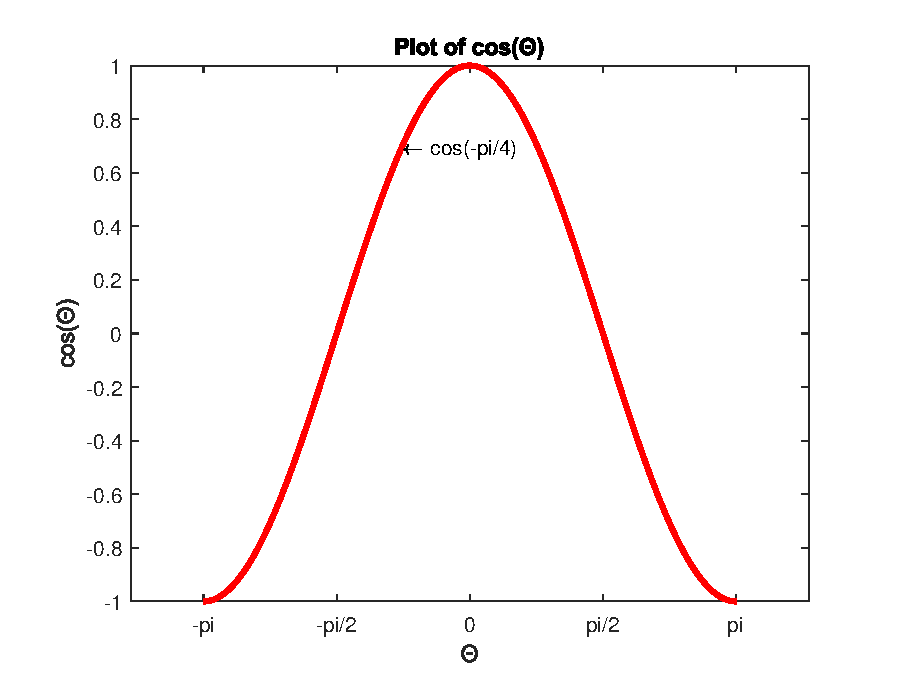
\includegraphics[width=.9\linewidth]{PlotOfCos.eps}\quad
            \\[\baselineskip]
            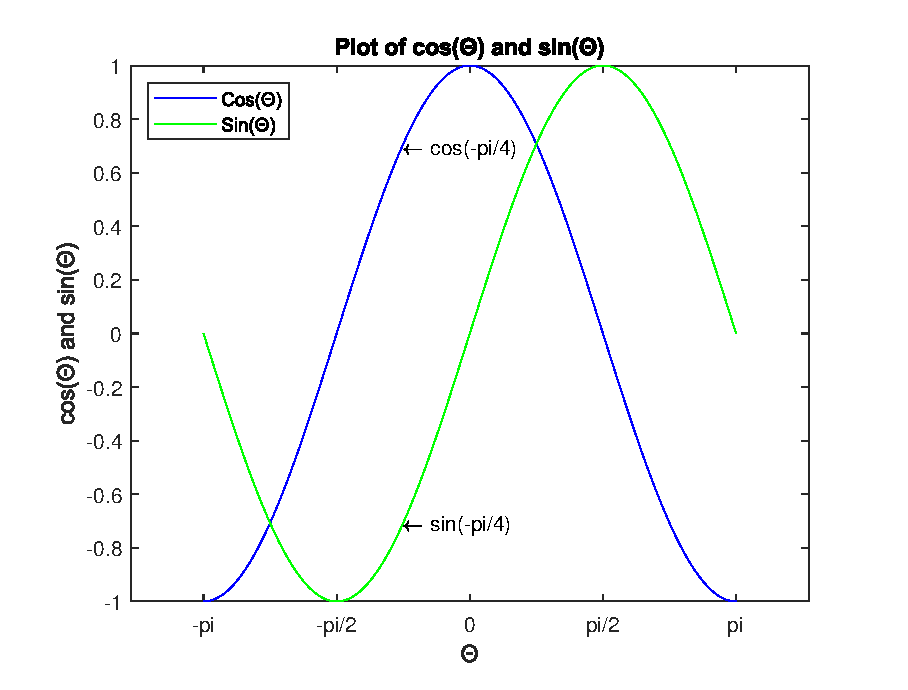
\includegraphics[width=.9\linewidth]{PlotOfCosAndSin.eps}\quad
        \end{center}
    
\end{document}